% -*- Mode:TeX -*-

%% IMPORTANT: The official thesis specifications are available at:
%%            http://libraries.mit.edu/archives/thesis-specs/
%%
%%            Please verify your thesis' formatting and copyright
%%            assignment before submission.  If you notice any
%%            discrepancies between these templates and the 
%%            MIT Libraries' specs, please let us know
%%            by e-mailing thesis@mit.edu

%% The documentclass options along with the pagestyle can be used to generate
%% a technical report, a draft copy, or a regular thesis.  You may need to
%% re-specify the pagestyle after you \include  cover.tex.  For more
%% information, see the first few lines of mitthesis.cls. 

%\documentclass[12pt,vi,twoside]{mitthesis}
%%
%%  If you want your thesis copyright to you instead of MIT, use the
%%  ``vi'' option, as above.
%%
%\documentclass[12pt,twoside,leftblank]{mitthesis}
%%
%% If you want blank pages before new chapters to be labelled ``This
%% Page Intentionally Left Blank'', use the ``leftblank'' option, as
%% above. 

\documentclass[12pt]{mitthesis}
\usepackage{lgrind}
\pagestyle{plain}

%% This bit allows you to either specify only the files which you wish to
%% process, or `all' to process all files which you \include.
%% Krishna Sethuraman (1990).

%% \typein [\files]{Enter file names to process, (chap1,chap2 ...), or `all' to
%% process all files:}
%% \def\all{all}
%% \ifx\files\all \typeout{Including all files.} \else \typeout{Including only \files.} \includeonly{\files} \fi

\begin{document}

% -*-latex-*-
% 
% For questions, comments, concerns or complaints:
% thesis@mit.edu
% 
%
% $Log: cover.tex,v $
% Revision 1.8  2008/05/13 15:02:15  jdreed
% Degree month is June, not May.  Added note about prevdegrees.
% Arthur Smith's title updated
%
% Revision 1.7  2001/02/08 18:53:16  boojum
% changed some \newpages to \cleardoublepages
%
% Revision 1.6  1999/10/21 14:49:31  boojum
% changed comment referring to documentstyle
%
% Revision 1.5  1999/10/21 14:39:04  boojum
% *** empty log message ***
%
% Revision 1.4  1997/04/18  17:54:10  othomas
% added page numbers on abstract and cover, and made 1 abstract
% page the default rather than 2.  (anne hunter tells me this
% is the new institute standard.)
%
% Revision 1.4  1997/04/18  17:54:10  othomas
% added page numbers on abstract and cover, and made 1 abstract
% page the default rather than 2.  (anne hunter tells me this
% is the new institute standard.)
%
% Revision 1.3  93/05/17  17:06:29  starflt
% Added acknowledgements section (suggested by tompalka)
% 
% Revision 1.2  92/04/22  13:13:13  epeisach
% Fixes for 1991 course 6 requirements
% Phrase "and to grant others the right to do so" has been added to 
% permission clause
% Second copy of abstract is not counted as separate pages so numbering works
% out
% 
% Revision 1.1  92/04/22  13:08:20  epeisach

% NOTE:
% These templates make an effort to conform to the MIT Thesis specifications,
% however the specifications can change.  We recommend that you verify the
% layout of your title page with your thesis advisor and/or the MIT 
% Libraries before printing your final copy.
\title{Automatic Protoboard Layout}

\author{Michael Mekonnen}
% If you wish to list your previous degrees on the cover page, use the 
% previous degrees command:
%       \prevdegrees{A.A., Harvard University (1985)}
% You can use the \\ command to list multiple previous degrees
%       \prevdegrees{B.S., University of California (1978) \\
%                    S.M., Massachusetts Institute of Technology (1981)}
\prevdegrees{B.S. EECS, Massachusetts Institute of Technology (2013) \\
             B.S. Mathematics, Massachusetts Institute of Technology (2013)}
\department{Department of Electrical Engineering and Computer Science}

% If the thesis is for two degrees simultaneously, list them both
% separated by \and like this:
% \degree{Doctor of Philosophy \and Master of Science}
\degree{Masters of Engineering in Electrical Engineering and Computer Science}

% As of the 2007-08 academic year, valid degree months are September, 
% February, or June.  The default is June.
\degreemonth{February}
\degreeyear{2014}
\thesisdate{\today}

%% By default, the thesis will be copyrighted to MIT.  If you need to copyright
%% the thesis to yourself, just specify the `vi' documentclass option.  If for
%% some reason you want to exactly specify the copyright notice text, you can
%% use the \copyrightnoticetext command.  
%\copyrightnoticetext{\copyright IBM, 1990.  Do not open till Xmas.}

% If there is more than one supervisor, use the \supervisor command
% once for each.
\supervisor{Dennis M. Freeman}{\textit{Professor}}
\supervisor{Adam J. Hartz}{\textit{Instructor}}

% This is the department committee chairman, not the thesis committee
% chairman.  You should replace this with your Department's Committee
% Chairman.
\chairman{\textit{Professor Albert R. Meyer}}{Chairman, Department Committee on Graduate Theses}

% Make the titlepage based on the above information.  If you need
% something special and can't use the standard form, you can specify
% the exact text of the titlepage yourself.  Put it in a titlepage
% environment and leave blank lines where you want vertical space.
% The spaces will be adjusted to fill the entire page.  The dotted
% lines for the signatures are made with the \signature command.
\maketitle

% The abstractpage environment sets up everything on the page except
% the text itself.  The title and other header material are put at the
% top of the page, and the supervisors are listed at the bottom.  A
% new page is begun both before and after.  Of course, an abstract may
% be more than one page itself.  If you need more control over the
% format of the page, you can use the abstract environment, which puts
% the word "Abstract" at the beginning and single spaces its text.

%% You can either \input (*not* \include) your abstract file, or you can put
%% the text of the abstract directly between the \begin{abstractpage} and
%% \end{abstractpage} commands.

% First copy: start a new page, and save the page number.
\cleardoublepage
% Uncomment the next line if you do NOT want a page number on your
% abstract and acknowledgments pages.
% \pagestyle{empty}
\setcounter{savepage}{\thepage}
\begin{abstractpage}
% $Log: abstract.tex,v $
% Revision 1.1  93/05/14  14:56:25  starflt
% Initial revision
% 
% Revision 1.1  90/05/04  10:41:01  lwvanels
% Initial revision
% 
%
%% The text of your abstract and nothing else (other than comments) goes here.
%% It will be single-spaced and the rest of the text that is supposed to go on
%% the abstract page will be generated by the abstractpage environment.  This
%% file should be \input (not \include 'd) from cover.tex.

As an important component of the Circuits module of the first Introduction to
Electrical Engineering and Computer Science course at MIT (6.01), students
design and
build several circuits over the course of three weeks. When working on the
more intricate circuits, an unfortunately large proportion of students' lab time
is spent on laying out the circuits on protoboards. This project introduces a
new circuit schematic entry tool for 6.01 capable of automatically generating
protoboard layouts for circuits that students may design in the course. The tool
allows for students to easily build and analyze circuit schematics through an
intuitive
graphical user interface, and automatically generates protoboard layouts that
are almost always easy to build and debug.
The layout problem is solved by utilizing the $A*$ search algorithm exactly as
presented in 6.01.

\end{abstractpage}

% Additional copy: start a new page, and reset the page number.  This way,
% the second copy of the abstract is not counted as separate pages.
% Uncomment the next 6 lines if you need two copies of the abstract
% page.
% \setcounter{page}{\thesavepage}
% \begin{abstractpage}
% % $Log: abstract.tex,v $
% Revision 1.1  93/05/14  14:56:25  starflt
% Initial revision
% 
% Revision 1.1  90/05/04  10:41:01  lwvanels
% Initial revision
% 
%
%% The text of your abstract and nothing else (other than comments) goes here.
%% It will be single-spaced and the rest of the text that is supposed to go on
%% the abstract page will be generated by the abstractpage environment.  This
%% file should be \input (not \include 'd) from cover.tex.

As an important component of the Circuits module of the first Introduction to
Electrical Engineering and Computer Science course at MIT (6.01), students
design and
build several circuits over the course of three weeks. When working on the
more intricate circuits, an unfortunately large proportion of students' lab time
is spent on laying out the circuits on protoboards. This project introduces a
new circuit schematic entry tool for 6.01 capable of automatically generating
protoboard layouts for circuits that students may design in the course. The tool
allows for students to easily build and analyze circuit schematics through an
intuitive
graphical user interface, and automatically generates protoboard layouts that
are almost always easy to build and debug.
The layout problem is solved by utilizing the $A*$ search algorithm exactly as
presented in 6.01.

% \end{abstractpage}

\cleardoublepage

\section*{Acknowledgments}

\textit{Acknowledgments.}
%%%%%%%%%%%%%%%%%%%%%%%%%%%%%%%%%%%%%%%%%%%%%%%%%%%%%%%%%%%%%%%%%%%%%%
% -*-latex-*-

% Some departments (e.g. 5) require an additional signature page.  See
% signature.tex for more information and uncomment the following line if
% applicable.
% % -*- Mode:TeX -*-
%
% Some departments (e.g. Chemistry) require an additional cover page
% with signatures of the thesis committee.  Please check with your
% thesis advisor or other appropriate person to determine if such a 
% page is required for your thesis.  
%
% If you choose not to use the "titlepage" environment, a \newpage
% commands, and several \vspace{\fill} commands may be necessary to
% achieve the required spacing.  The \signature command is defined in
% the "mitthesis" class
%
% The following sample appears courtesy of Ben Kaduk <kaduk@mit.edu> and
% was used in his June 2012 doctoral thesis in Chemistry. 

\begin{titlepage}
\begin{large}
This doctoral thesis has been examined by a Committee of the Department
of Chemistry as follows:

\signature{Professor Jianshu Cao}{Chairman, Thesis Committee \\
   Professor of Chemistry}

\signature{Professor Troy Van Voorhis}{Thesis Supervisor \\
   Associate Professor of Chemistry}

\signature{Professor Robert W. Field}{Member, Thesis Committee \\
   Haslam and Dewey Professor of Chemistry}
\end{large}
\end{titlepage}


\pagestyle{plain}
  % -*- Mode:TeX -*-
%% This file simply contains the commands that actually generate the table of
%% contents and lists of figures and tables.  You can omit any or all of
%% these files by simply taking out the appropriate command.  For more
%% information on these files, see appendix C.3.3 of the LaTeX manual. 
\tableofcontents
\newpage
\listoffigures
\newpage
\listoftables


%% This is an example first chapter.  You should put chapter/appendix that you
%% write into a separate file, and add a line \include{yourfilename} to
%% main.tex, where `yourfilename.tex' is the name of the chapter/appendix file.
%% You can process specific files by typing their names in at the 
%% \files=
%% prompt when you run the file main.tex through LaTeX.

% Chapter for introduction.

\chapter{Introduction}
\label{ch:intro}

\section{Problem Statement}

In this paper we discuss the problem of automatic protoboard layout generation.
Importantly, we are interested in automatically generating layouts that are
easy to build, easy to debug, and aesthetically pleasing. The tool this
paper discusses
is strictly geared towards circuits that students would build in the
Introduction to Electrical Engineering and Computer Science I\cite{sixohone} 
course at MIT (also known as 6.01).

We are motivated to solve the layout
problem in order to let 6.01 students spend more of their lab time thinking
about how to design
circuits and less time thinking about how to lay them out on protoboards.
In this project we built\footnote{The tool was implemented entirely in the
Python programming language.}
a tool that lets students easily build and
simulate circuit schematics through an intuitive graphical user interface (GUI).
After building and testing a circuit schematic with the tool, a student can
proceed to building the circuit on a physical protoboard based on the layout
generated by the tool. Not only does the tool generate a layout, but it
also makes it easy to relate the original schematic drawn by the student to the
generated layout. With this tool, a student's lab time will be spent mostly
on designing, building, and testing circuits rather than on the difficult and
arguably less instructive task of layout.

\section{Outline}

Chapter \ref{ch:background} describes in detail the terminology that will be
used in this paper and explores the current infrastructure available for
6.01 students as well as previous work done in automatic layout generation.
Chapter \ref{ch:methods} discusses how we solved the problem, including various
alternatives considered in each part of the solution, and how we evaluated
our solution. Chapter \ref{ch:results} presents data to compare the various
alternatives discussed in Chapter \ref{ch:methods} and also evaluates the final
algorithm on a large test dataset. Finally, Chapter \ref{ch:discussion}
presents arguments for the choices made in our solution to the problem and
also elaborates upon the results presented in Chapter \ref{ch:results}.

% This is an example of how you would use tgrind to include an example
% of source code; it is commented out in this template since the code
% example file does not exist.  To use it, you need to remove the '%' on the
% beginning of the line, and insert your own information in the call.
%
%\tagrind[htbp]{code/pmn.s.tex}{Post Multiply Normalization}{opt:pmn}


% Chapter for background.

\chapter{Background}
\label{ch:background}

In this chapter we discuss essential background information to this project.
First, we discuss the specific terminology used in this paper. Next, we discuss
previous work done that relates to this project.

\section{Technical Background}

As we are producing a new teaching tool for 6.01 in this project,
let us first discuss the scope of circuits in 6.01.

\subsection{Circuit Components}

The rudimentary circuit components used in 6.01 are resistors, operational
amplifiers (op-amps), and potentiometers (pots). In addition to these basic
parts, students may build circuits to control LEGO motors or to control
aspects of robots designed specifically for 6.01. One of the 6.01 robots is
depicted in Figure \ref{fig:robot}. The robots can be equipped with heads that
contain three parts held together by a shaft: a LEGO motor, a potentiometer, and
a plate containing two photosensors. The robot in Figure \ref{fig:robot} has a
head attached. To connect a layout to a LEGO motor, a student would use a 6-pin
connector, and to connect a layout to a robot or a robot head, a student
use an 8-pin connector.

All together, the circuit pieces that may be used in constructing protoboard
layouts in 6.01 are resistors, op-amps, pots, (6-pin) motor connectors, (8-pin)
robot connectors, and (8-pin) head connectors.

\begin{figure}
\begin{center}
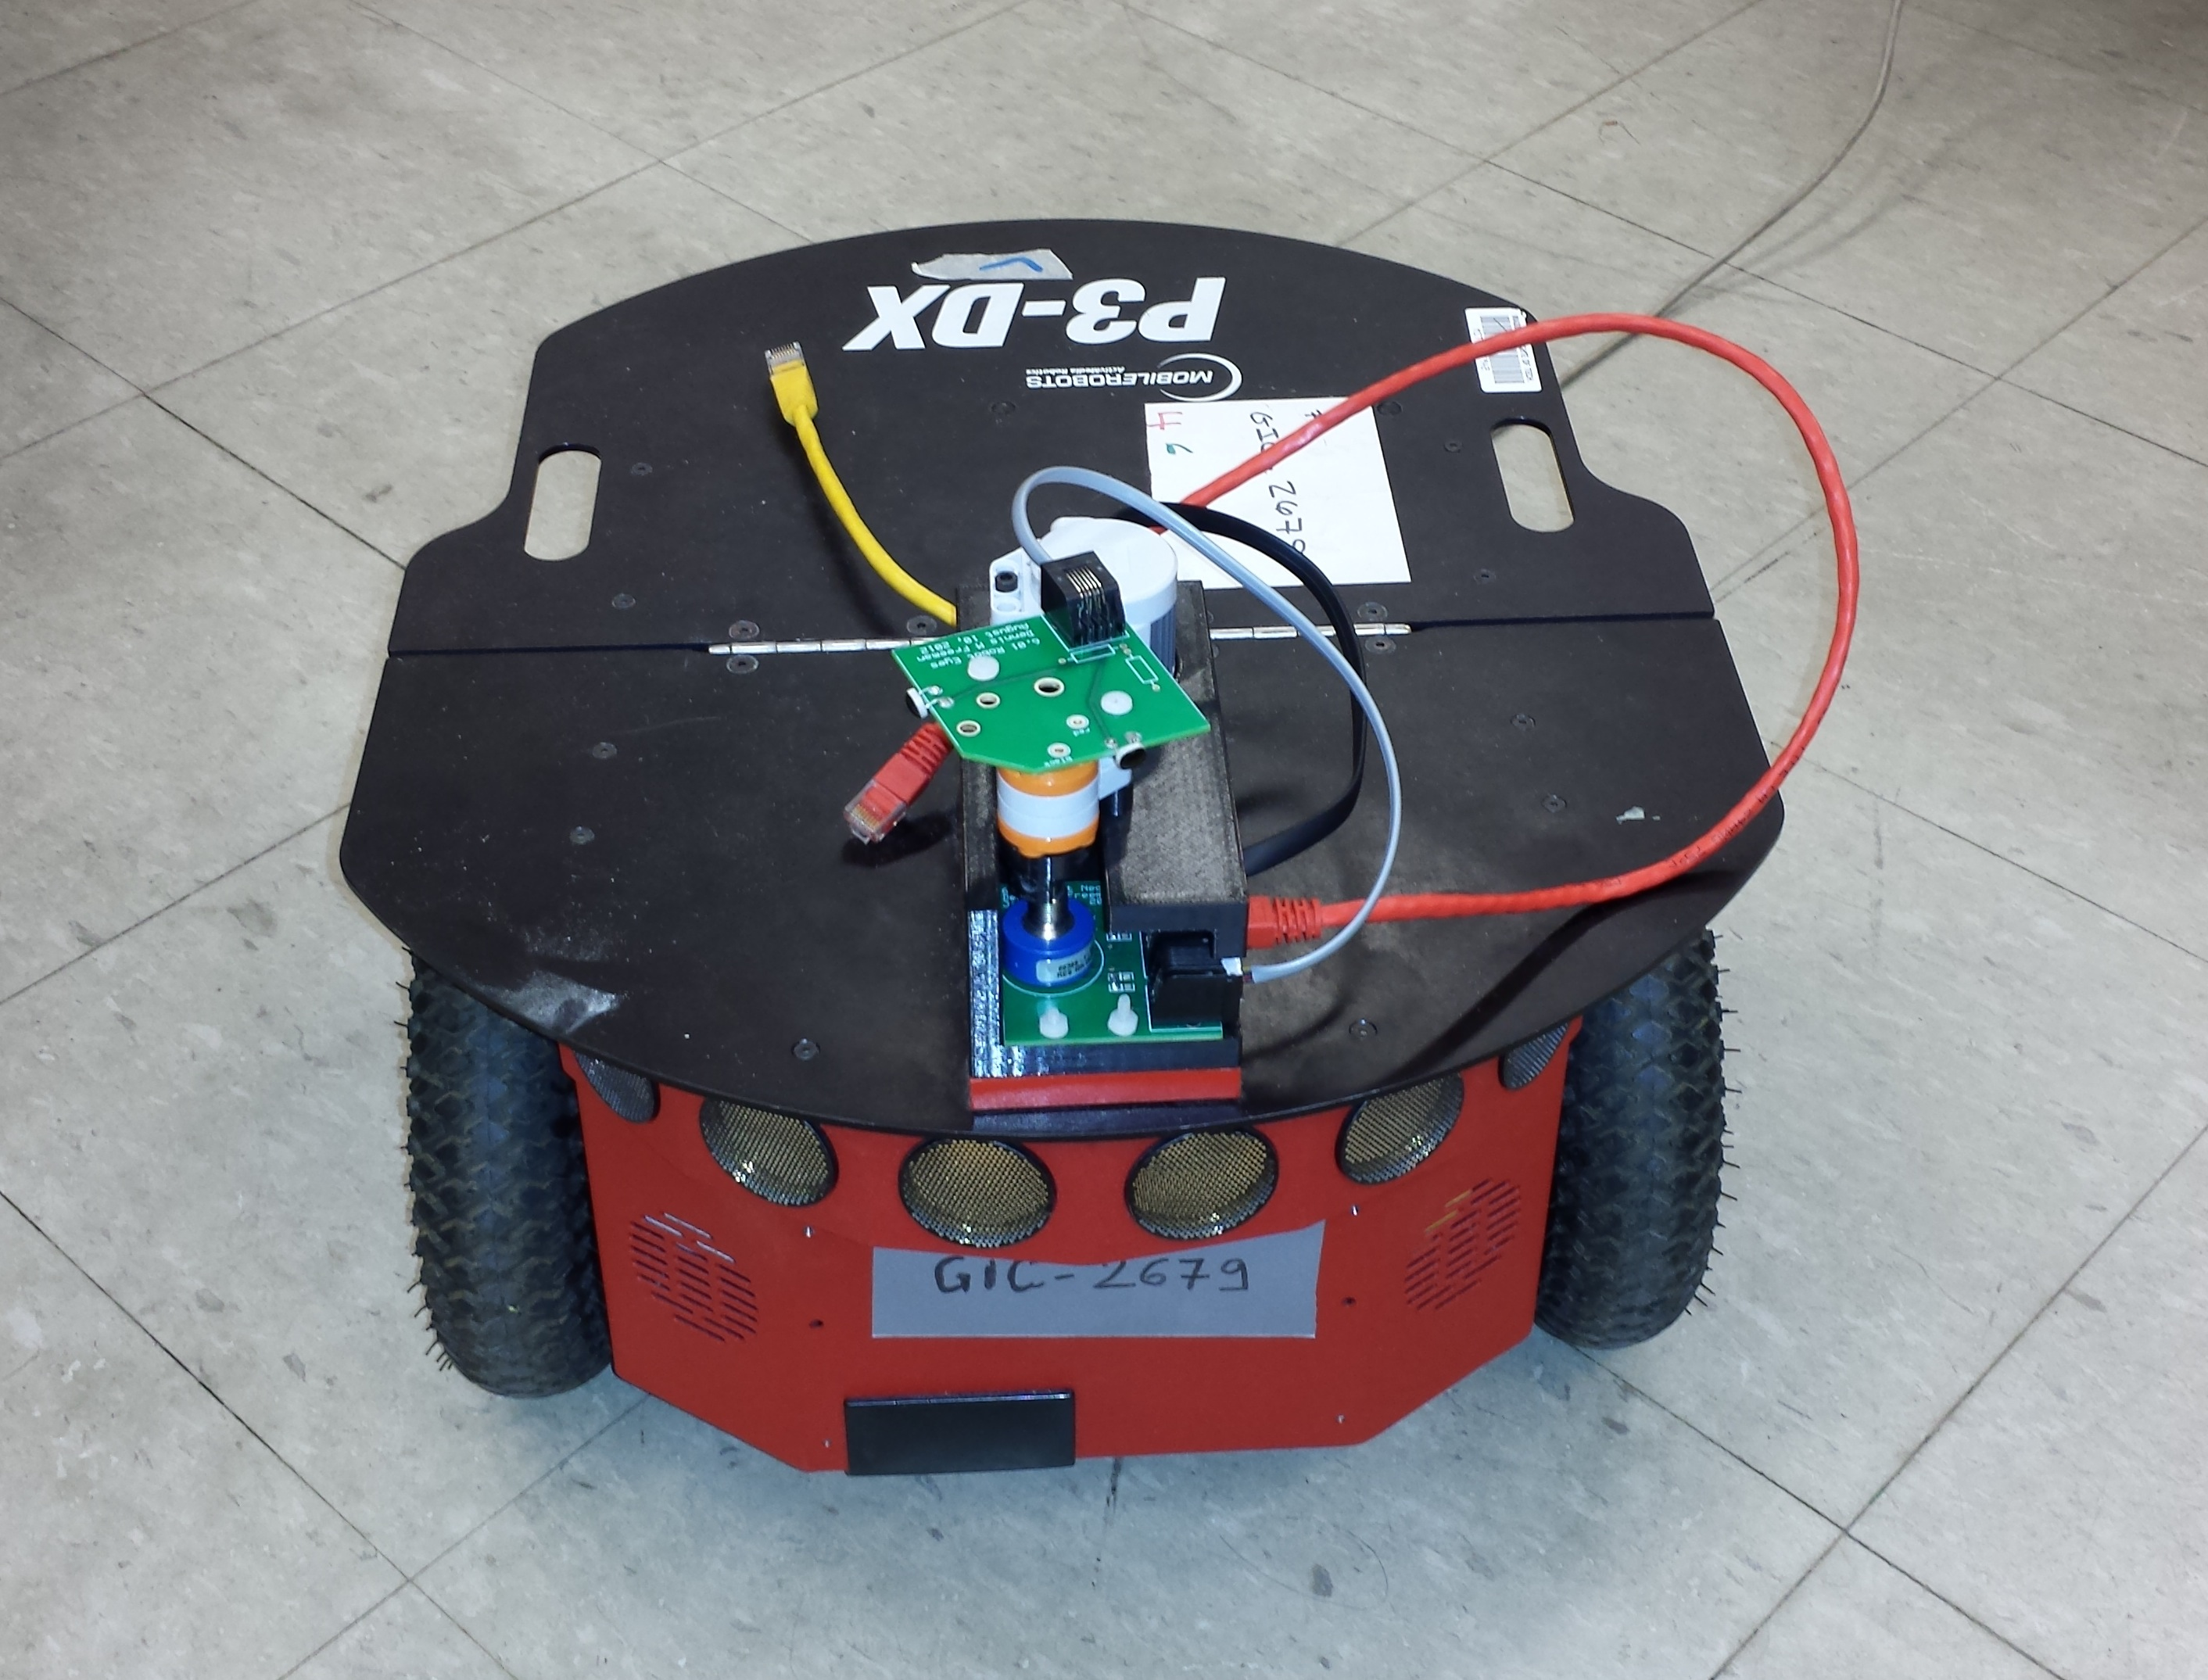
\includegraphics[width=\textwidth]{Images/robot.jpeg}
\caption[6.01 robot]{One of the 6.01 robots, with a head attached.}
\label{fig:robot}
\end{center}
\end{figure}

\subsection{Circuit Schematic}

Throughout this paper, the term \textit{circuit schematic} will refer to a
drawing or a sketch of a circuit containing its components and all the
interconnections between the components drawn as wires. This is what one would
sketch on a piece of paper in the process of designing a circuit. Figure
\ref{fig:schematic} presents an example of a circuit schematic.

\begin{figure}
\begin{center}
\includegraphics[width=\textwidth]{sample_schematic-22.mps}
\caption[Sample circuit schematic]{Sample schematic of a motor angular position
controller circuit.}
\label{fig:schematic}
\end{center}
\end{figure}

\subsection{Protoboard}
\label{sec:what_is_protoboard}

Protoboards are boards on which one can quickly build and test
small circuits. They present a $2$-dimensional array of interconnected dots
in which circuit pieces and wires can be inserted. Figure
\ref{fig:physical_protoboard} presents an example of an empty physical
protoboard. In
the orientation depicted in Figure \ref{fig:physical_protoboard}, a protoboard
has $4$ groups of rows: the first $2$ rows, the next $5$ rows, the next $5$
rows, and finally the last $2$ rows. In the first and last groups, the dots on
the protoboard are interconnected horizontally. In the middle
two groups, the dots are interconnected vertically. This
interconnection scheme is depicted in Figure \ref{fig:physical_protoboard}.

\begin{figure}
\begin{center}
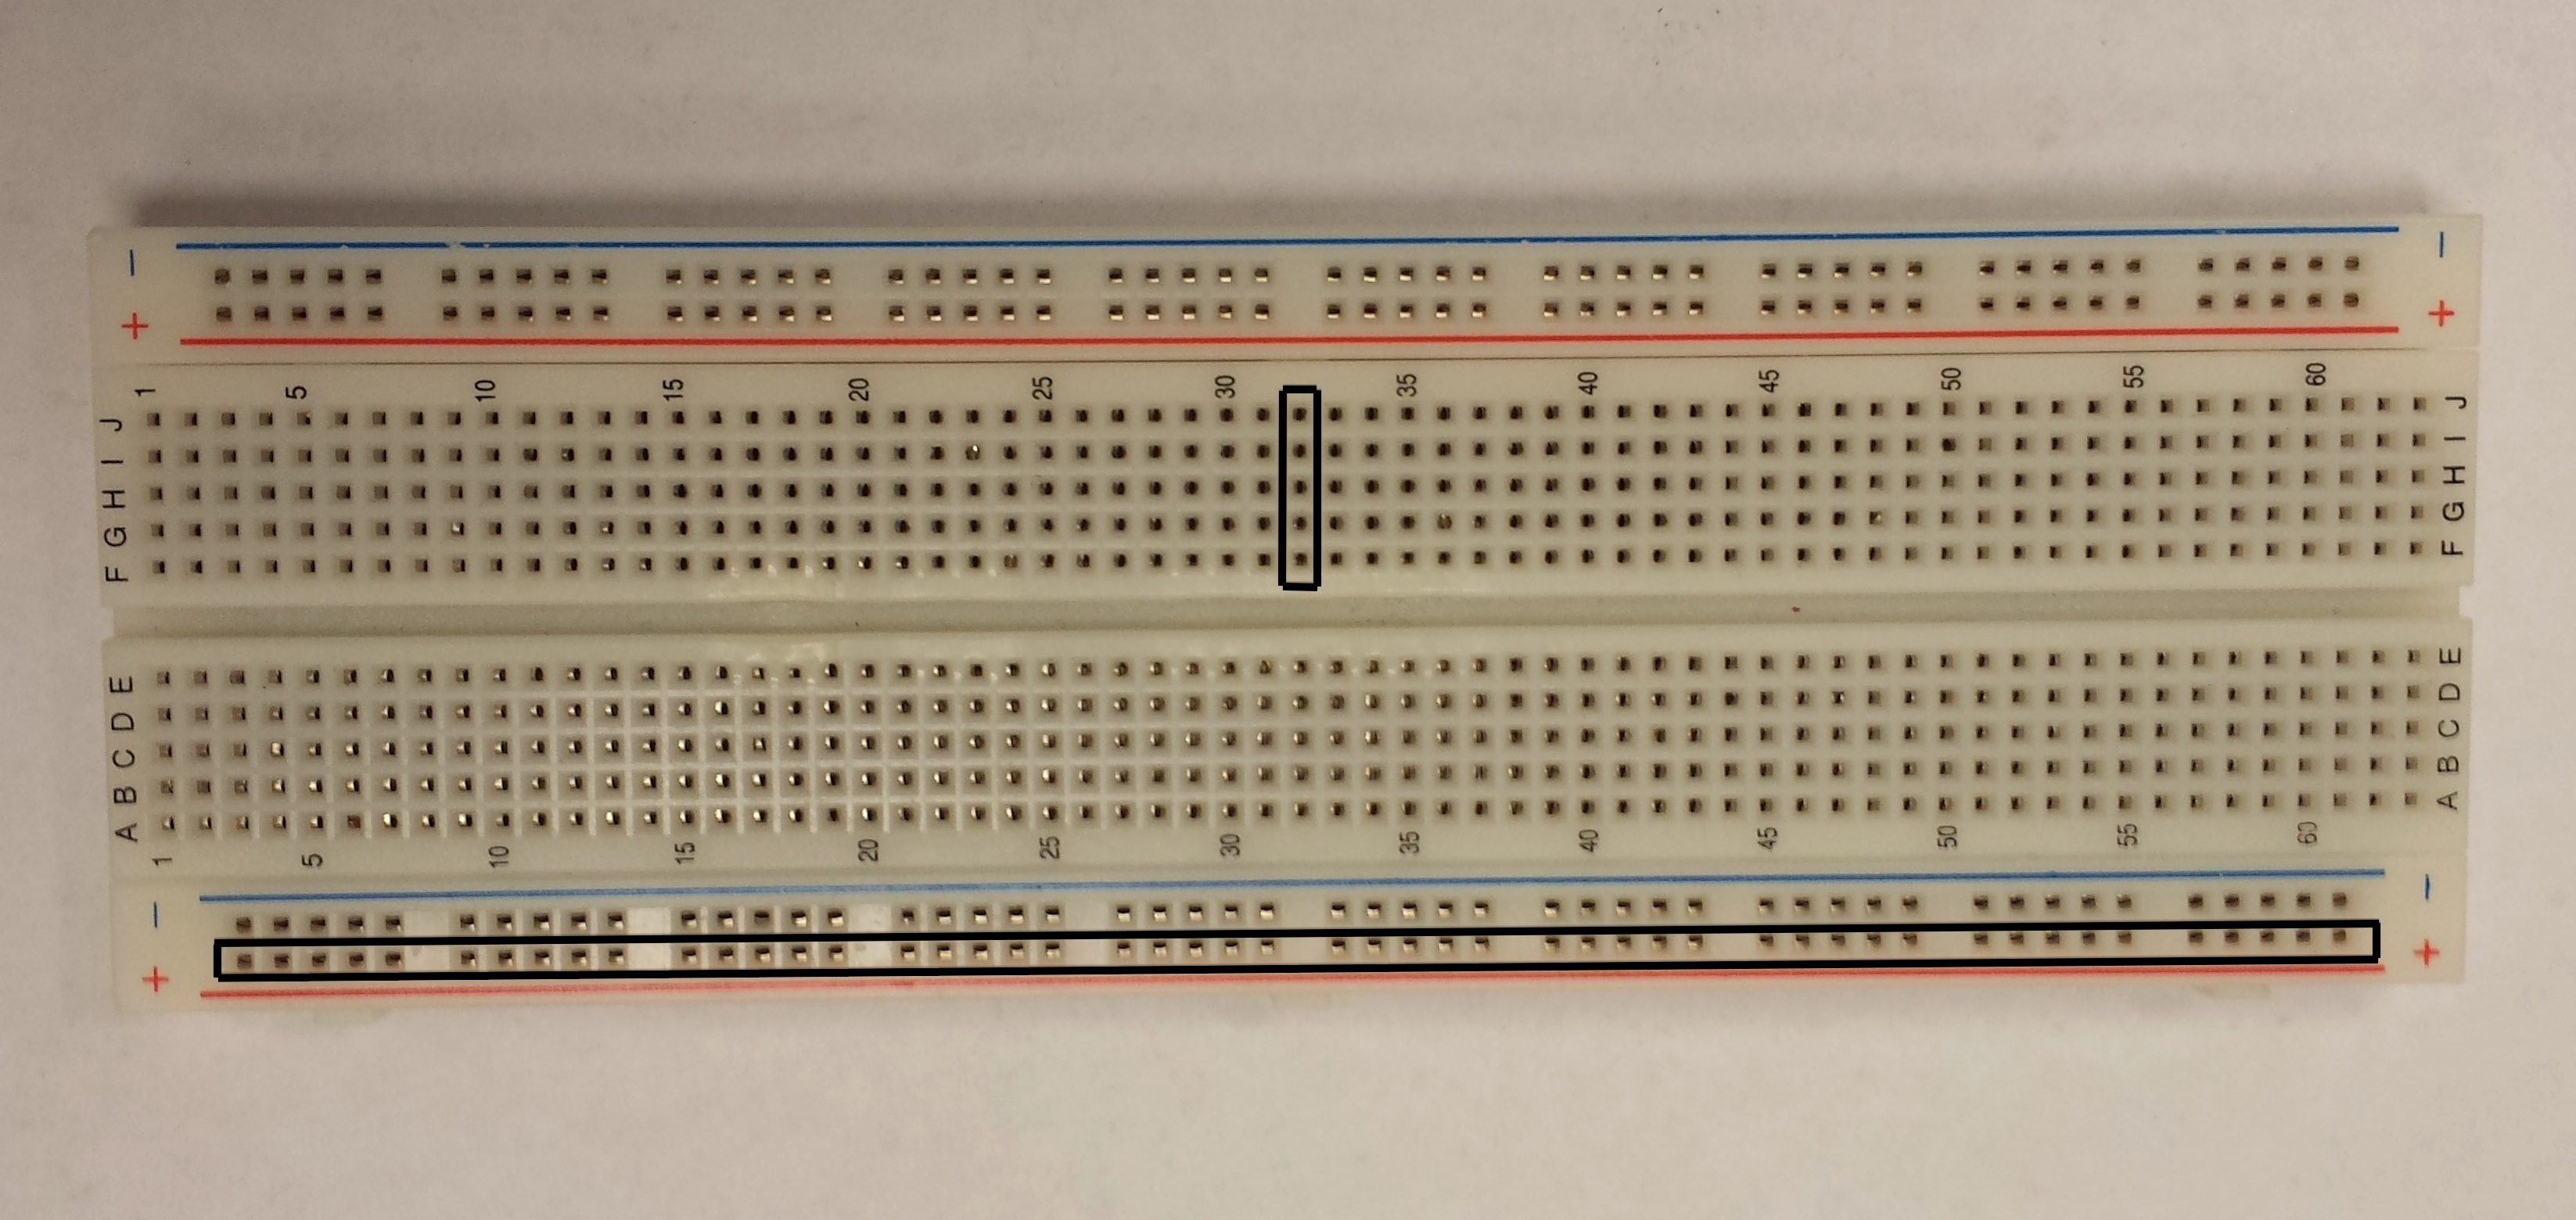
\includegraphics[width=\textwidth]{Images/physical_protoboard.jpg}
\caption[Protoboard]{A protoboard. In the top and bottom groups of rows,
the dots are internally interconnected horizontally.
In the middle two groups, the dots are interconnected vertically.}
\label{fig:physical_protoboard}
\end{center}
\end{figure}

\subsection{Protoboard Layout}

The protoboard layout of a given schematic is the placement of circuit pieces
and wires on a protoboard that corresponds to the schematic. This is done by
placing the appropriate pieces on the protoboard and then appropriately
interconnecting them with wires as prescribed by the schematic. As an example,
Figure \ref{fig:eg_s_to_pb} presents one possible protoboard layout
corresponding to the schematic shown in Figure \ref{fig:schematic}.

\begin{figure}
\begin{center}
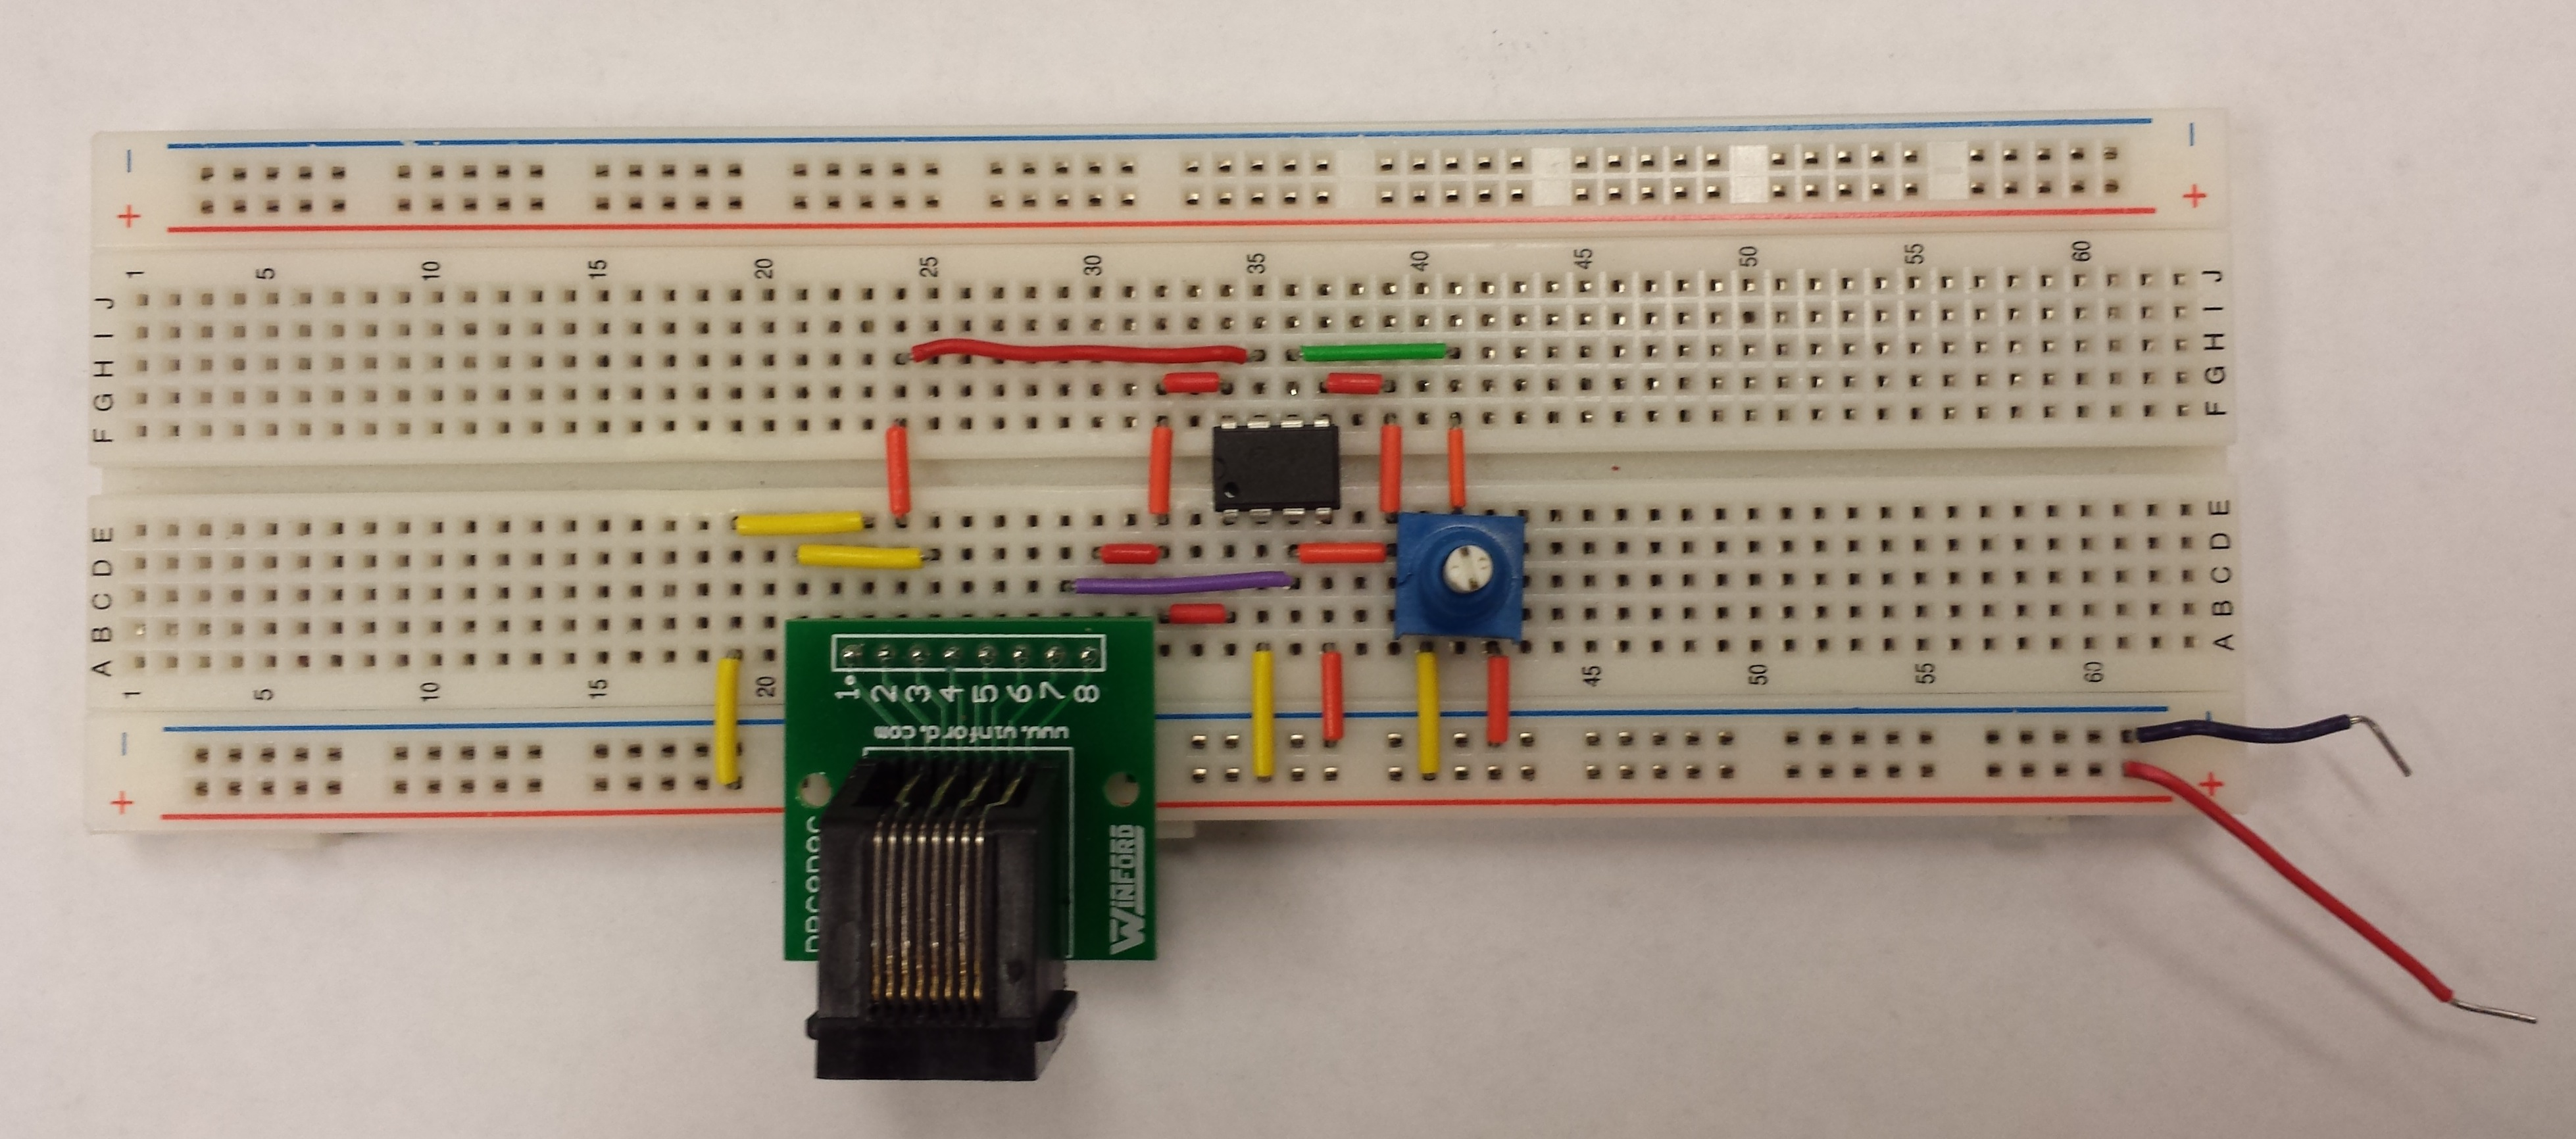
\includegraphics[width=\textwidth]{Images/sample_physical_layout.jpg}
\caption[Sample protoboard layout]{Protoboard layout for the schematic shown in
Figure \ref{fig:schematic}.}
\label{fig:eg_s_to_pb}
\end{center}
\end{figure}

For each of the circuit components we are interested in, there is a corresponding
circuit piece that may be inserted into the protoboard. The one exception is that
op-amps come in pairs. That is, each op-amp circuit piece that is inserted in the
protoboard actually contains two op-amp components within it. This raises an
important design problem when laying out a schematic - the need to find a
good way to group together the op-amps in a schematic to result in a ``good''
layout. To solve this problem, the designer must have some criteria for what
makes a layout ``good.'' While there are no conclusive answers to this
question, keeping in mind that we want layouts that are easy to build,
easy to debug, and aesthetically pleasing, we could come up with the
following rules of thumb:
\begin{itemize}
\item The layout should not have any wires that cross circuit pieces.
\item The layout should have no crossing wires, especially occlusions (i.e.
crossing wires with the same orientation).
\item The layout should only have horizontal and vertical wires (i.e. no
diagonal wires).
\item The layout should have as few wires as possible.
\item The total length of wires in the layout should be as small as possible.
\end{itemize}

Given the background information discussed thus far, the goal of this project is
automatically generating a ``good'' protoboard layout from a circuit schematics.

\section{Previous Work}

Here we will discuss previous work that has been done relating to this project.
First, as our project aims to augment the quality of 6.01, we look at the
currently available infrastructure. Next, we look at what work has
been done relating to layout in general.

\subsection{CMax}

In a typical circuits lab in 6.01, students first design their circuits by
drawing schematics of the circuits on paper.
After iteratively improving their designs based on discussions with staff
members, they build their circuits on a simulation tool called Circuits Maximus
(CMax)\cite{cmax}.
With CMax, a student can lay out a circuit on a simulated protoboard, and test
the circuit to make sure that it behaves as desired. CMax provides a very fast
and safe way of debugging circuit layouts compared to debugging layouts on a
physical protoboard. Once the students are satisfied with their
observations from CMax, they build their circuits on physical protoboards and
carry out the appropriate experiments. Figure \ref{fig:cmax_sample} presents a
CMax layout of the schematic in Figure \ref{fig:schematic}.

\begin{figure}
\begin{center}
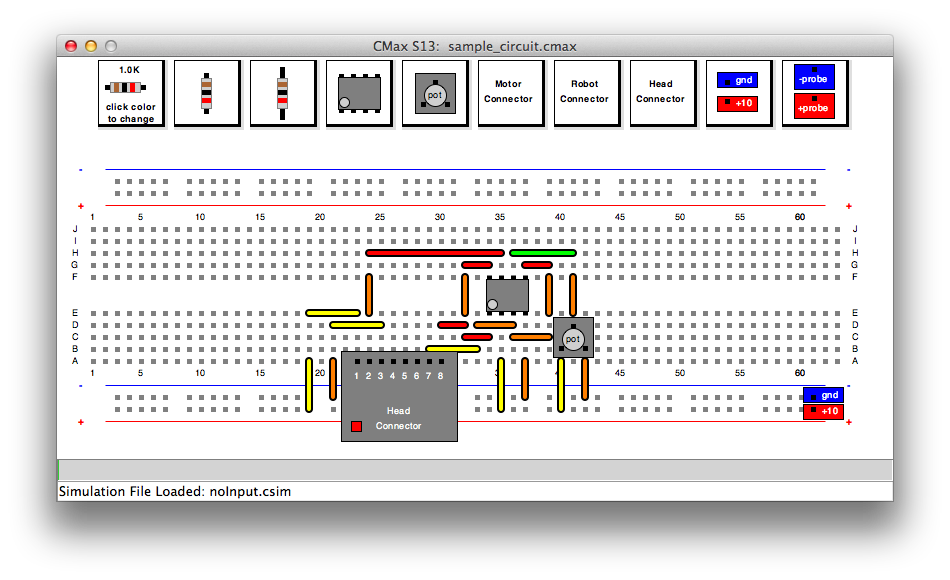
\includegraphics[width=\textwidth]{Images/sample_circuit.png}
\caption[CMax]{CMax layout for the schematic shown in Figure
\ref{fig:schematic}.}
\label{fig:cmax_sample}
\end{center}
\end{figure}

Using CMax has reduced circuit debugging time for 6.01 students.
Its introduction has made
learning circuits significantly easier for many students, especially those that
have little or no prior experience with circuits. In addition to making the lab
exercises more manageable, it provides students with a handy way to
build, analyze, and experiment with circuits at their own leisure outside of lab.

While CMax is a fantastic tool, a tool that can automate the layout process
can be even more useful. The most instructive part of the labs that students do
in the circuits
module of 6.01 is really designing the circuits in the first place, which they
currently do by drawing schematic diagrams on paper. Once they are happy with
their schematic diagrams, they proceed to laying out the corresponding circuits
with CMax. The process of laying out a schematic does not really have very much
instructive substance. This process is essentially solving a puzzle, and has
almost nothing to do with the subject matter -- designing circuits. In fact,
when the circuits get complicated and involve many pieces, translating a
schematic diagram into a protoboard layout gets to be quite challenging and
time-consuming. In these situations, students often end up with convoluted and
unpleasant layouts that are very difficult to debug in the likely case of the
circuit not behaving as expected. Not only are such layouts difficult to debug
for the students themselves, but they are also often difficult for staff
members to understand. In the best case scenario, students should have to work
out the right schematic diagram of the circuit of interest, but should not have
to produce the corresponding protoboard layouts.

With the schematic entry tool this paper introduces, a typical 6.01 circuits lab
would proceed as follows. First, as before, the students would draw schematic
diagrams of their circuits on paper. Once they have
schematic drawings they are happy with, they can directly draw their schematic
drawings on the schematic entry tool. In fact, students may proceed directly to
building the schematic drawings on the tool, bypassing the
experimentation on
paper. Once they have a schematic drawn, they can analyze it with the tool,
discuss it with staff members, and improve it easily and quickly with
the tool. When they are
satisfied with the behaviors of their schematic circuit, they can produce the
corresponding protoboard layout automatically. The automatic generation of
protoboard layouts would be
the most important advantage of this tool. They can then build the layout on a
physical protoboard and carry out experiments with it.

\subsection{Current work in automatic layout}

In my explorations, I was not able to find any tools that completely
automatically translate circuit schematics into protoboard layouts.
However, there
do exists tools that perform partially- or fully-automatic Printed Circuit
Board (PCB) layout. To my findings, most of these tools do not publish their
algorithms and, rather, keep them proprietary. Hence, I was not able to build my
work off of any existing products. In a sense, this project aims to build
something new.

% Chapter for evaluation method.

\chapter{Evaluation}

\textit{How are we going to evaluate a particular solution to the problem?}

% Chapter for alternative methods to solving the problem.

\chapter{Methods}
\label{ch:methods}

In this Section, I discuss my solution to the problem and various alternatives I
considered along the way.

\section{Overview}

I solved this problem by formulating it as a search problem. By this I mean,
given a schematic of a circuit, I start from an empty protoboard, and I search
through the space of all possible protoboard layouts to find the protoboard
corresponding to the schematic at hand. The space of all possible protoboards is
very large \q, so I utilize various simplifications
and heuristics to facilitate the search.

I broke down the problem into two parts. The first task is finding a placement
of all the circuit pieces on the protoboard. The second task is wiring them up
appropriately.

\section{Part 1: Piece Placement}
\label{sec:placement}

Let us first consider how to place a set of circuit pieces on the protoboard for
a given circuit schematic. Any given circuit may contain resistors, Op Amps,
pots, motors, head connector parts, or robot connector parts. For each of these
components, we must put down a corresponding piece on the protoboard. As each
piece may be placed on the protoboard in one of many different ways, I first
decided on a fixed set of allowed placements for each of the pieces. Figure
\ref{fig:piece_placement} presents these acceptable placements.
Resistors are placed in the middle strip of the protoboard. Op Amp pieces are
also placed in the middle strip of the protoboard, but with two possible
orientations. Op Amp pieces are unique in that each Op Amp pieces contains two
Op Amps within it. Thus, we face the task of packaging the Op Amps in the
schematic in the ``best" possible way, i.e. so as to require as little work as
possible when wiring the pieces together. Section \ref{sec:justify_placement}
more precisely discusses the number of possibilities. Pots have two possible
vertical positions (TODO: this is wrong!) as well as two possible orientations.
The connector pieces have two possible vertical positions each.

\begin{figure}
\begin{center}
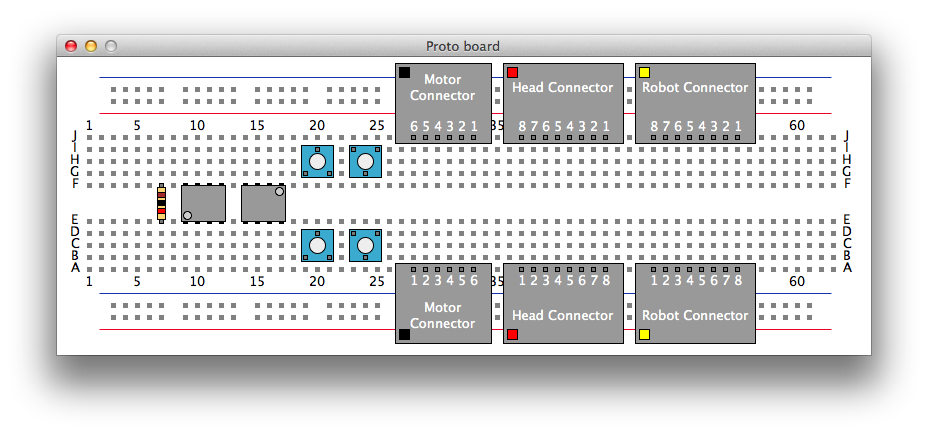
\includegraphics[width=\linewidth]{Images/piece_placement_options.png}
\caption{Various acceptable ways of putting each of the circuit pieces on the
protoboard.}
\label{fig:piece_placement}
\end{center}
\end{figure}

\subsection{Choosing a Placement}

When choosing a placement of circuit pieces on the protoboard, we have at hand a
plethora of options. First we must choose among a possibly large number of ways
to package together the Op Amps in the circuit. For each possible packaging of
Op Amps, we must consider various ways of placing the pieces on the protoboard,
even with the restrictions put forth above.

\subsubsection{Simplifications}

I reduce this large number of options by only allowing placements in which no
two pieces share a column. This is not necessary in general, but the
number of pieces necessary for a typical 6.01 circuit would certainly fit in
this framework.

Next, I specify that there be exactly two columns on the protoboard separating
each consecuitive pair of pieces, unless the pieces are both resistors, in which
case there must be exactly one column separating them. These numbers of columns
were chosen to leave enough space for wiring. Given a set of pieces to be put on
the protoboard, this specification reduces the
problem of choosing a placement for the pieces to finding an \emph{order} of the
pieces together with choosing their respective vertical locations and
orientations.

Given these simplifications, we have various options as to how to pick a
placement.

\subsubsection{Random Placement}

One simple alternative may be to choose a placement randomly. That is, we choose
an Op Amp packaging randomly; we choose an order of the pieces randomly; and we
choose the vertical locations and orientations of the pieces randomly as well.
The advantage of this
approach is that it gives us a placement very quickly without requiring much
computation. On the other hand, we may end up placing two pieces that need to be
connected to each other very far apart, and we will have a difficult time doing
the wiring. Hence, we ought to consider alternatives in which we take into
account the task of wiring. We should try to place the pieces so as to require
as little work during wiring as possible.

\subsubsection{Minimal Heuristic Cost}

The key idea is that if two pieces are meant to be connected together by wires,
then they ought to be placed close to each other on the protoboard. We can
capture this idea by assigning heuristic costs to the placements and choosing
a placement that produces the minimal heuristic cost.

Let us first devise the cost function to achieve this goal. Given a circuit
schematic and a corresponding placement of the circuit pieces on the protoboard,
what do we need to connect with wires? Well, every pair of components in the
schematic that are connected by a wire gives us a corresponding pair of
locations on the protoboard that ought to be connected by wires. However, we can
express this requirement a little bit more concisely. We ought to consider all
of the nodes in the schematic, and find the circuit components in the schematic
that are connected to the respective nodes. Now for each node in the circuit, we
get a set of locations on the protoboard that ought to be interconnected. The
first step in devising the cost function we are looking for is to have a way to
estimate the cost of connecting two locations on the protoboard. A simple such
cost function that comes to mind is the Manhattan distance between the two
locations. Recall that we want to produce aesthetically pleasing protoboard
layouts, and one of the requirements in achieving this goal is only using
horizontal and vertical wires (i.e. no diagonal wires) so the Manhattan distance
cost is appropriate. Given this heuristic cost for connecting two locations with
wires, we can define the heuristic cost for interconnecting the locations
associated with a particular node to be the weight of the minimum spanning tree
of the locations. Now we can define the cost of a placement to be the sum over
all nodes in the circuit of the cost for interconnecting the locations for each
node.

Now that we have a cost function for placements, we can aim to find a
placement with the minimal cost. However, this involves trying all possible
orderings of the pieces with which we are working. For example, if we are trying
to order $10$ pieces, we would need to look at $10! = 3628800$ possible
orderings \q. Note that this is in addition to
searching over all possible ways
of packaging the Op Amps together. It is clear to see that the search for a
minimal cost placement quickly gets out of hand. So we aim to find a placement
that has a very small, though maybe not minimal, cost.

\subsubsection{Small Heuristic Cost}

Algorithm \ref{alg:small_cost_placement} presents a polynomial-time procedure
that orders a
given list of pieces in a way that results in a small cost. The algorithm places
one of the pieces at a time, starting from an empty placement. It relies
on two ideas. First, once a piece has been placed, all the pieces that are
connected to it will be placed soon after so that it is more likely that those
pieces are placed close to it. Second, we place the pieces with the most nodes
first since those are the ones that most likely have connections with many other
pieces.

\begin{algorithm}
\KwData{A list $P$ of circuit pieces.}
\KwResult{A list $R$ of circuit pieces representing a placement.}
\BlankLine
Sort $P$ in decreasing number of nodes on the respective pieces\\
$Q$ $\leftarrow$ empty Queue\\
$R$ $\leftarrow$ empty List\\
\While{$P$ is not empty}{
Pop the first piece in $P$ and push it onto $Q$\\
\While{$Q$ is not empty}{
$p$ $\leftarrow$ $Q$.pop()\\
Consider all vertical locations and orientations of $p$\\
Place $p$ at an index in $R$ that minimizes the cost of $P$\\
\ForEach{piece $q$ in $P$ connected to $p$}{
Pop $q$ out of $P$ and push it onto $Q$\\
}}}
\caption{Producing a circuit piece placement with small heuristic cost.}
\label{alg:small_cost_placement}
\end{algorithm}

Using one of the above methods, we can find a placement of circuit pieces on a
protoboard. Our next task is wiring them together to produce a circuit
equivalent to the circuit schematic of interest.

\section{Part 2: Wiring}

In the previous section we discussed what locations we need to wire together:
for every node in the circuit, we get a set of locations on the protoboard that
need to be interconnected. The question now is how to achieve this wiring. We
approach the problem as a search problem and use the $A*$ search algorithm to
solve it.

\subsection{Using $A*$}

When using the $A*$ algorithm, we need to design four things:

\begin{enumerate}
\item The notion of a vertex\footnote{The prefered name is ``node" but I will
use vertex since we already use node to refer to nodes in circuits.} in the
search tree, the cost associated with a vertex, and how we obtain the neighbors
of a vertex,
\item The starting vertex,
\item How we identify whether a particular vertex in the search tree achieves
the goal of the search, and
\item A heuristic function that estimates the distance from a given vertex to a
goal vertex.
\end{enumerate}

\subsection{Vertices}

Each vertex will hold a representation of some protoboard. Each representation
will contain all of the pieces, and possibly a set of wires interconnecting the
pieces. The starting vertex will have all of the pieces but no wires.

We obtain the neighbors of a vertex by taking the current protoboard and
producing new ones in which we place exactly one wire at various locations. We
choose the starting point of a wire to be any one of the free locations on the
protoboard that is already connected to one of the pieces, and we extend the
wires in all possible vertical and horizontal directions up to some fixed wire
length. Note that we need
to take great care when placing wires in order not to short different nodes. We
discard any vertices that arise from placing a wire that shorts two different
nodes.

The way we define the cost of a vertex, i.e. the cost of getting from the
starting vertex to a vertex of interest, depends on what we consider to be an
aesthetically pleasing protoboard layout. In general, we want to penalize having
long wires, many wires, or crossing wires. In my implementation, while I have
a large penalty for two crossing wires of opposite orientations (i.e. vertical
and horizontal), I do not allow crossing wires that have the same orientation as
this configuration is particularly difficult to physically build and debug.
Finally, we want to favor making a desired interconnection between locations
on the protoboard. I chose my penalties experimentally
\q.

Each vertex will not only hold a protoboard, but it will also hold a set of
pairs of locations on the protoboard that need to be connected by wires. Each
pair $(loc_1, loc_2)$ of locations tells us that we need to have a set of wires
connecting some location connected to $loc_1$ to some location connected to
$loc_2$.

An important consideration we need to make is how we want to organize the
search. Recall that we have a set of nodes in the circuit of interest, and for
each node we have a set of locations that need to be interconnected. Given this
information, we may choose one of the following three strategies to carryout the
search:

\begin{enumerate}
\item For each node, collect a set of pairs of locations on the protoboard
corresponding to a minimum spanning tree of the locations for that node, so that
if all pairs of locations in this spanning tree are connected, then the
locations for the node will be interconnected. Collect all such pairs of
locations for all of the nodes in the circuit, and have the starting vertex hold
this set of pairs of locations.
\item Treat each node separately. That is, iteratively interconnect the
locations for each of the nodes until there are no more nodes in the circuit.
\item Treat each pair of locations that needs to be connected separately. That
is, iteratively connect pairs of locations that need to be connected until there
are no more pairs.
\end{enumerate}

The choice of one of these strategies has a significant effect on the outcome of
the search. We will discuss the difference in detail in Chapter
\ref{ch:results}.

\subsection{Goal test}

Given a vertex, we know that it is a goal vertex if all of the pairs of
locations it holds are already connected in the protoboard it holds.

\subsection{Search heuristic}

In $A*$ search, choosing the right heuristic can often make the search much more
efficient. In our problem, one option we have is not to use a heuristic, and
that alternative will be explored in Chapter \ref{ch:results}. However there is
a natural heuristic that suggests itself that we ought to consider. Given a
vertex, we can estimate its distance from a goal as follows. For each pair of
locations $(loc_1, loc_2)$ that need to be connected, we could consider its
distance from the
goal to be the smallest Manhattan distance between any location connected to
$loc_1$ and any other location connected to $loc_2$. To compute the heuristic
cost of a vertex, we simply add up this value for each of the pairs of locations
that need to be connected. Chapter \ref{ch:results} presents the performance of
this heuristic verses using no heuristic.

\section{Treating Resistors as Wires}
\label{sec:resistors_as_wires}

The discussion in Section \ref{sec:placement} presented that we treat
resistors just as we do the other components. That is, we give each resistor a
fixed place on the protoboard in the first step of the algorithm before the
wiring step. However, resistors have the special property among the circuit
pieces that they can be thought of as wires of length $3$.
Hence, it may be possible to handle resistors in the wiring step instead of the
placement step. Chapter \ref{ch:results} presents a comparison of these two
approaches.

Note that treating resistors in the wiring step is not a trivial task. First,
there may be nodes in the circuit that are connected to some resistors, but no
other pieces. In this case, we must be sure to reserve space on the protoboard
for that node as the wiring step relies on the presence of each node on the
protoboard. Second, we must keep careful track of pairs of locations that need
to be connected by simple wires and pairs of locations that need to be connected
using resistors.

\section{Evaluation Method}

Here we present how we go about evaluating a particular solution to the problem.
How can we tell if a layout tool is good? In particular, how can we tell if a
layout tool is good enough for the purposes of 6.01 labs. To answer these
questions well, we need to test the layout tool on numerous schematics and
analyze its performance on laying out those schematics. As manually generating
numerous test schematics is tedious and very time-consuming, we devised a method
to randomly generate thousands of test schematics.

The random schematic generation goes as follows. We create $6$ basic sub-parts
of schematics. These $6$ bases are depicted in Figure
\ref{fig:random_gen_bases}. These bases cover all of the components that may be
necessary in a 6.01 circuit. Each sub-part also offers at least $3$ points of
connection with other subparts. The random generation algorithm takes all
possible combinations of
$6$ bases, allowing for repetition of bases with some restictions.
The Head Connector and Robot Connector bases can appear at most once as there is
no need for more than one of each of these in 6.01 labs. The pot-follower base (
i.e. the base that contains one pot and a follower op amp) can appear at most
twice as we never need more than two pots in 6.01 circuits. The motor base can
also appear at most twice as we never need more than two motors per circuit in
6.01 labs. The other bases, T-resistor configuration and voltage divider, can be
repeated up to 6 times. For a given combination of bases, we generate up $n$
schematics, where $n$ dependes on the number of bases in the configurations (
larger for configurations with more bases in them).
We generate the $n$ schematics by choosing a number of interconnections between
the bases from $0$ to $n-1$. For each number of interconnections, we generate
a schematic in which we put that many randomly chosen wires interconnecting
the bases in the combination. Figure \ref{fig:example_random_schematic} presents
a sample randomly generated schematic.

This scheme produces a total of $4425$ test schematics out of a possible total
of approximately $1.2e27$. When testing a particular algorithm on these test
schematics, we run the algorithm on each test schematic $10$ times. Chapter
\ref{ch:results} presents the data collected in this manner comparing the
various alternatives discussed in this Chapter.

\begin{figure}
\begin{center}
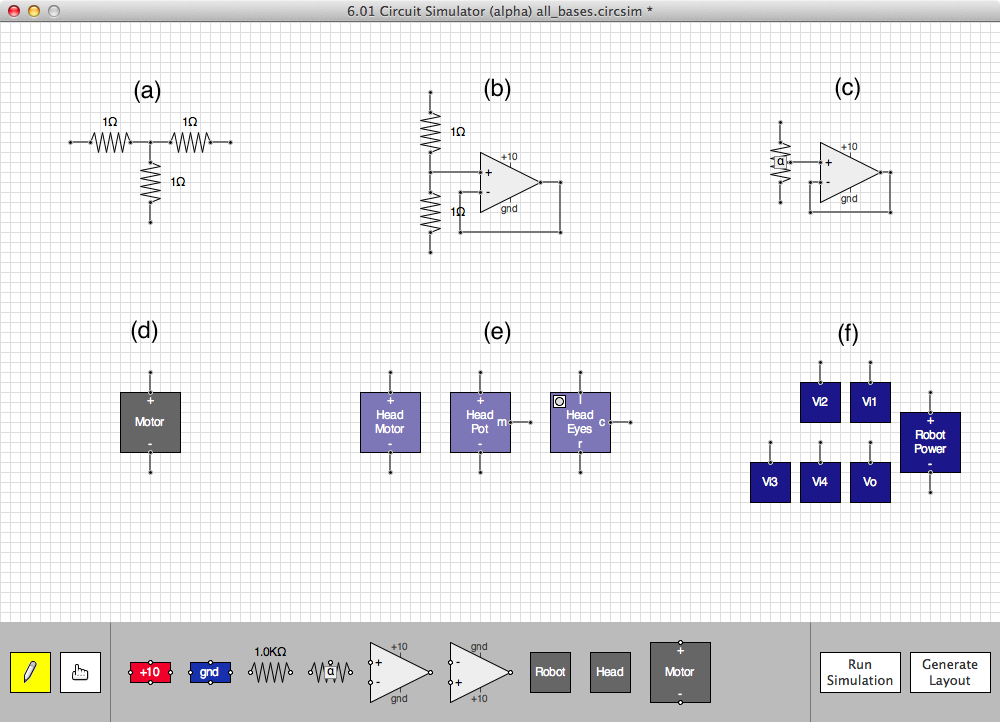
\includegraphics[width=\textwidth]{Images/auto_generation_bases.png}
\caption{Bases for random schematic generation.}
\label{fig:random_gen_bases}
\end{center}
\end{figure}

\begin{figure}
\begin{center}
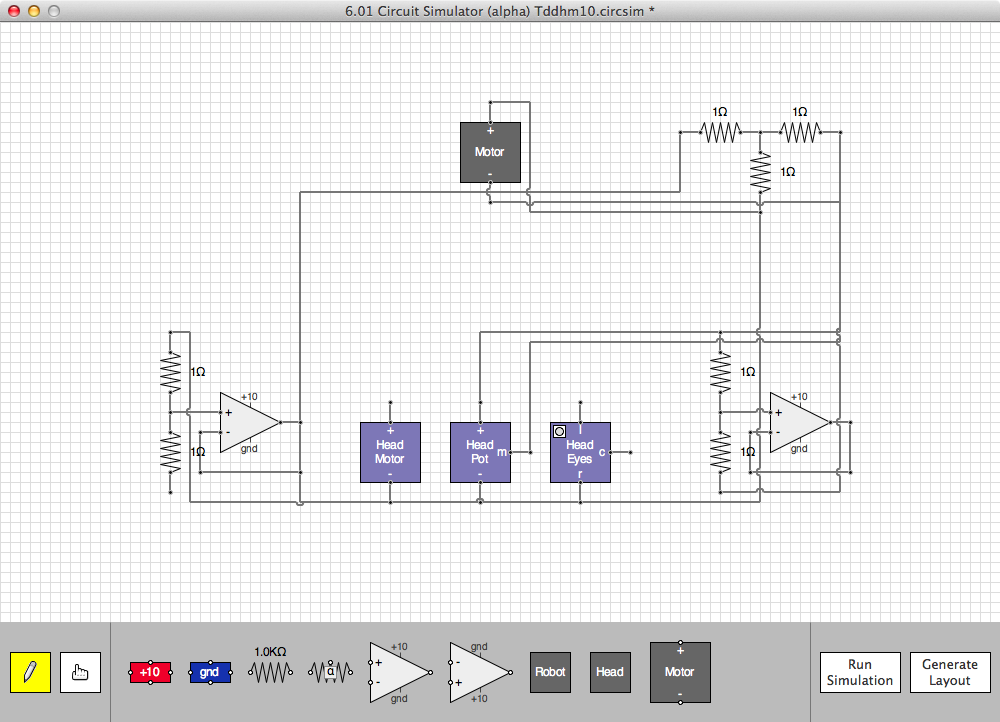
\includegraphics[width=\textwidth]{Images/auto_generation_example.png}
\caption{Sample randomly generated schematic.}
\label{fig:example_random_schematic}
\end{center}
\end{figure}

% Chapter in which we explore how well various approaches do.

\chapter{Results}
\label{ch:results}

\textit{Quantitatively compare the various methods discussed in the previous
section.}

% Chapter where we explain the results.

\chapter{Discussion}
\label{ch:discussion}

In this section we provide justifications for the choices made in solving the
protoboard layout problem, and also detailed analysis of the data presented in
Chapter \ref{ch:results}.

\section{Justifying Placement Choices}
\label{sec:justify_placement}

\subsubsection{Resistors}

For the sake of simplicity, and to significantly reduce the search space
\q, for every resistor in the schematic, I use one resistor piece on the
protoboard placed in the middle strip of the protoboard as shown in Figure
\ref{fig:piece_placement}. This choice, i.e. allowing the resistor pieces to
only reside in the middle strip of the protoboard, is critical
as the resistor pieces can generally be placed at numerous places on the
protoboard.
With this restriction, there are $63$ slots available for one resistor. Without
this restriction, there are a total of $763$ slots available. The restirction is
good when we consider the reduction in the search space size. On the other hand,
the restriction is bad when we
consider the size of circuits the algorithm can layout. Given that the number
of resistors in a typical 6.01 circuit is very
small \q, this restriction proves to be very useful.

\subsubsection{Op Amps}

Op Amps are the trickiest components to handle because each Op Amp package put
on the protoboard contains two Op Amps within it. Equation
\ref{eq:opamp} presents an expression for the value $f(n)$, the number of
different ways to package together $n$ Op Amps. For example, if we have $2$ Op
Amps, we can either use one Op Amp package for each, or put them both in the
same package, which we can do in one of two different ways. Hence, $f(2) = 3$.
To get a sense of how many different packagings are possible, Table
\ref{tb:opamp} gives the values of $f(n)$ for various $n$.

\begin{equation}
f(n) = \sum\limits_{k=0}^{\lfloor\frac{n}{2}\rfloor}{\frac{n!}{k!(n - 2k)!}}
\label{eq:opamp}
\end{equation}

\begin{table}
\begin{center}
\begin{singlespace}
\begin{tabular}{c | c}
$n$ & $f(n)$ \\
\hline
\hline
1 & 1 \\
2 & 3 \\
3 & 7 \\
4 & 25 \\
5 & 81 \\
6 & 331 \\
7 & 1303 \\
8 & 5937 \\
9 & 26785 \\
10 & 133651
\end{tabular}
\end{singlespace}
\end{center}
\label{tb:opamp}
\caption{Number of ways of packaging together $n$ Op Amps for various values of
$n$.}
\end{table}

Our placement approach explores all possible ways
of packaging up the Op Amps. We do this because the typical 6.01 circuit contains
no more than $6$ Op Amps, and so we are tasked with exploring at most $331$
alternatives, which doesn't happen to be too computationally intensive. If the
algorithm was meant to handle a larger number of Op Amps (for example $10$), then
this approach would be silly, and we would have to resort to perhaps considering
the packagings that require the fewest number of Op Amps to make a choice.

\subsubsection{Pots}

Each pot piece can be placed in one of two vertical locations on the protoboard.
Each pot piece also has two possible orientations. TODO: really 6 different
vertical locations.

\subsubsection{Head, Motor, and Robot Connectors}

Our choices for the connector pieces is certainly one of the two presented in
Figure \ref{fig:piece_placement}. Any other placement of the connector pieces
would unecessarily take up valueable rows.

\section{Explaining the Results}

Chapter \ref{ch:results} presented quantitative data to compare the various
alternatives we have in solving the protoboard layout problem. Here, we will
analyze that data and give reasonings for why we obtained the results
that we obtained. For each comparison, we present exemplar layouts generated
by the alternative methods for the schematic shown in Figure
\ref{fig:exemplar_schematic}.

\begin{figure}
\begin{center}
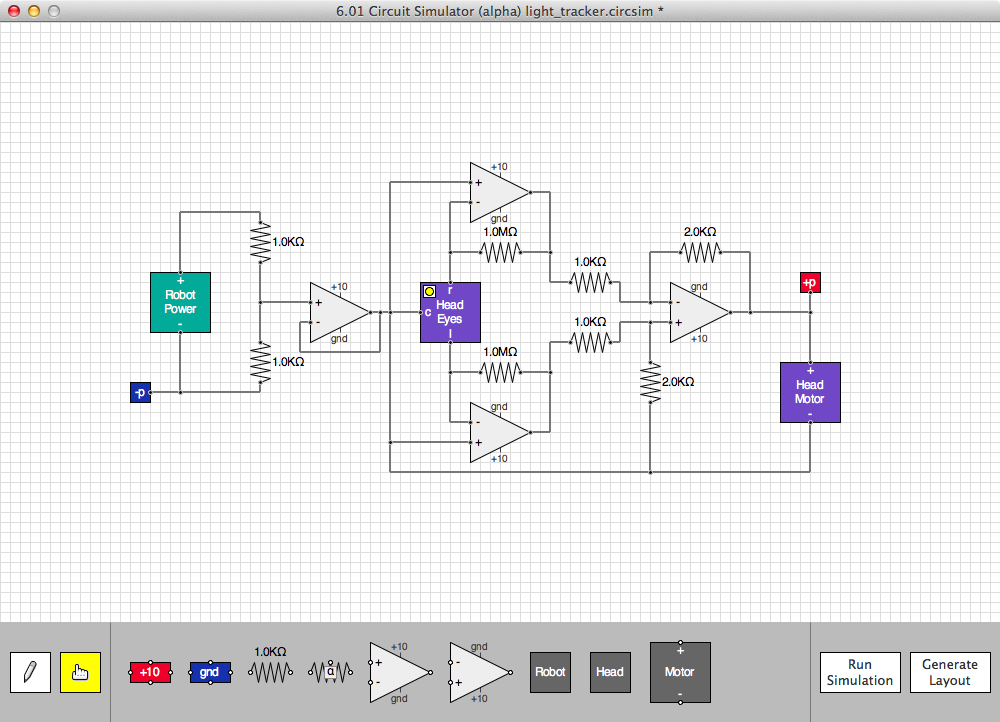
\includegraphics[width=\textwidth]{Images/exemplar_schematic.png}
\caption{Exemplar schematic.}
\label{fig:exemplar_schematic}
\end{center}
\end{figure}

\subsection{Comparing placement methods}

In Figure \ref{fig:placement_success} and Table \ref{tb:placement_success} we
see that the distance method exceeds the blocking method in number of circuits
solved $10$ times out of $10$ as well as in the number of circuits solved $0$
to $2$ times out of $10$. On the other hand, the blocking method exceeds the
distance method in number of circuits solved from $3$ to $9$ times out
of $10$. If our primary goal is avoiding failure, then these results suggest
that the blocking method is a better placement method. If, on the other hand,
our primary goal is being consistent on success (while not necessarily being
successful), then these results perhaps suggest that the distance method is
better. In a sense, these results suggest that while the blocking method
generally produces placements that are easier for the wiring stage, it has more
variability in the placements it produces for the same circuit. The distance
method, on the other hand, produces worse placements (i.e. placements that are
harder to wire), but has much less variability. This observation from the data
makes intuitive sense as there are likely to be more placements that are minimal
in blocking rows than placements that minimize pairwise distances between pairs
of protoboard locations that need to be connected.

Despite the important differences presented above, it is interesting to note
that the
success rates of the two placement methods are not that different form each
other. Looking at the percentages given in Table \ref{tb:placement_success}, we
see that the success rates are very comparable.

When we consider success rate as a function of the complexity of circuits, we
reach some interesting patterns. From Figure \ref{fig:placement_success_trend} we
can gather that when the number of pins in the circuit is less than roughly $26$,
the blocking method generally has a higher success rate, but when the number of
pins is greater than $26$, the success rates of the two methods are very
comparable. This suggests that the blocking method is a better placement method
for the less complex circuits, but does not do any better on the more
complex ones. These results compliment what we found above. These results
suggest that the blocking method generally produces placements that are easy to
wire. These placements are easy in that the search in wiring is less likely to
get stuck while trying to connect a pair of locations. This is precisely a result
of the fact that the blocking method attempts to free as many rows as possible.
The blocking method is less effective on the more complex circuits because
despite freeing rows, it may ask for elaborate connections to be made, i.e.
connections between distant pairs of locations on the protoboard. The distance
method, on the other hand, attempts to avoid this problem by trying to minimize
the distances between the locations that need to be connected. Hence we would
not expect the blocking method to be better on the more complex circuits.
Interestingly, it does not seem to be worse on the more complex circuits either.

As we would expect, we certainly observe that as the complexity of the circuits
increases, success rate generally decreases for both of the placement methods.
The curves in Figure \ref{fig:placement_success_trend} seem to shoot back up
at the far end of the figure, but this is a result of the fact that there are
very few circuits at that end of the figure, on which the algorithm happened to
be consistently successful. It is important to note, once again, that the success
rates for the two placement methods are very comparable despite the difference
discussed above.

Let us now consider wiring time as the basis for comparison. Once again, in
Figure \ref{fig:placement_time_trend} we notice a very interesting separation
at roughly $26$ pins per circuit. When the number of pins in the circuits is
less than $26$, the wiring times for the two methods are very comparable.
When the number of pins in the circuits is greater than $26$, however, the
blocking methods consistently takes longer. This is very much related to the
discussion above that the blocking method may often ask for elaborate connections
to be made. As the complexity of circuits increases, the blocking method will
require the wiring step to make more elaborate connections than would the distance
method. Hence, when we are using the blocking method and the algorithm does succeed,
we would certainly expect the wiring step to take longer than if we had used the
distance method.

As we would expect, we certainly see that as the complexity of the circuits
increases, the amount of time spent by the wiring step also increases. As we did
for the success rate trends as a function of circuit complexity, we observe that
there are outliers at the far end of the figure due to a very small sample of the
most complex circuits in the randomly generated schematic dataset.

Finally, let us look at layout complexity as the basis for comparison. Figure
\ref{fig:placement_quality_trend} presents graphs that compare numbers of wires,
numbers of wire crosses, and total wire lengths. We first observe that the
number of wires used by the two methods are almost identical. As the complexity
of the circuit increases, we see that the blocking method uses more wires than
does the distance method, but by and large the values are very comparable. This
makes intuitive sense as we are rarely required to use more wires than
absolutely necessary (keeping wires horizontal and vertical) to connect a pair
of locations (?). When we look at the number of wire crosses in the layouts, we
see that the blocking method consistently results in more wire crosses. Similarly,
when we look at the total length of wires used in the layouts, the blocking
method exceeds the distance method consistently, with the difference getting
higher as complexity increases. This can be explained by the fact that the
blocking method may require elaborate connections, especially as the circuits
get more complex.

It is difficult to conclusively pick a better placement method from these results.
It is clear that both methods have their strengths and weaknesses. In Section
\ref{sec:method_combination} we will discuss how combining these two methods can
get us the best of both worlds (?).

\begin{figure}
\begin{center}
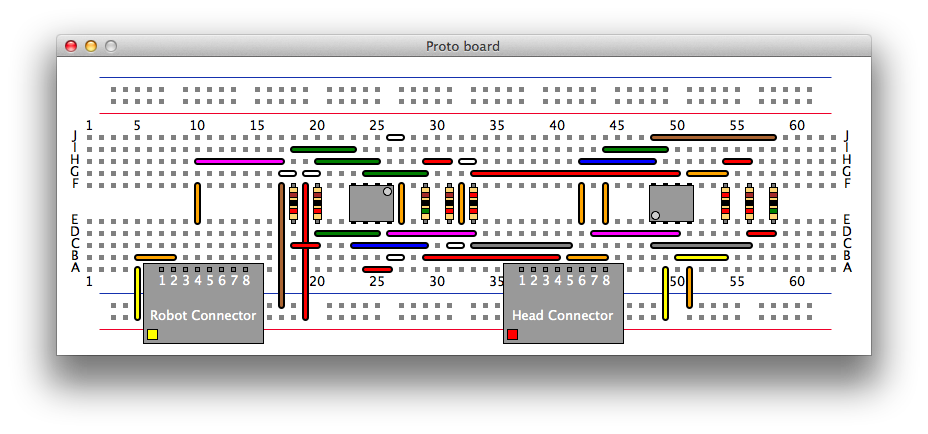
\includegraphics[width=\textwidth]{Images/exemplar_per_pair_decreasing.png}
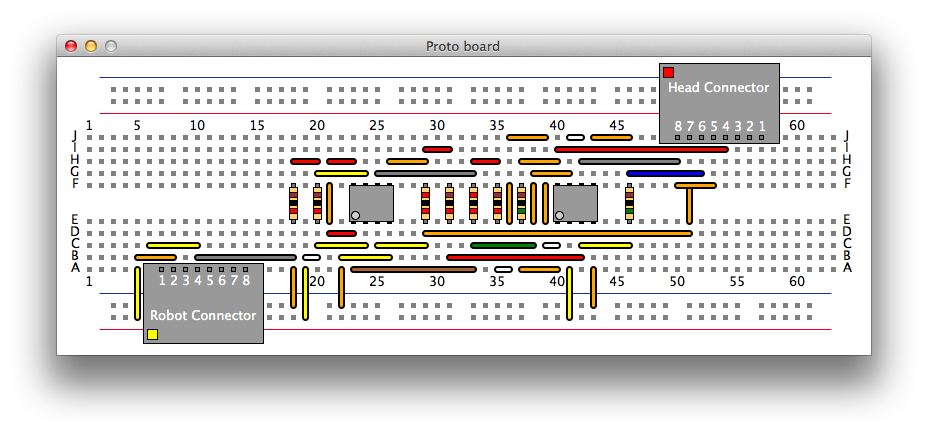
\includegraphics[width=\textwidth]{Images/exemplar_distance.png}
\caption{Blocking vs. Distance.}
\end{center}
\end{figure}

\subsection{Comparing wiring methods}

To compare the wiring methods, let us start with the success rate for each method.
Figures \ref{fig:wiring_success} and \ref{fig:wiring_success_trend}, and Table
\ref{fig:wiring_success} provide the appropriate data. The very first fact we
observe is that the all-pairs method has a much smaller success rate than all of
the other alternatives, especially as circuit complexity increases. The reason
for this, in large part, is the fact that we impose a cutoff on the number of
nodes to expand in the search (TODO: this must be discussed in Methods). As we
are using just the one search to connect all pairs of locations, the search
cutoff would be expected to have more of an effect on the all-pairs method. The
other four alternatives have very comparable success rates.

Next we look at Figure \ref{fig:wiring_time_trend} to compare wiring times for
the five methods. Once again, we observe that the all-pairs methods takes
significanlty more time than the other methods. When attempting to connect all
pairs in one search, the method searches for an appealing layout, which may
require searching through a large number of alternatives, especially for more
complex circuits. Hence, we would expect the all-pairs methods to generally take
more time than the other alternatives. We also observe from Figure
\ref{fig:wiring_time_trend} that the wiring times for the two per-node methods
are comparable, and that the wiring times for the two per-pair methods are also
comparable, but that the per-node wiring times are generally bigger than the
per-pair wiring times. This trend is also expected as the per-node methods
attempt to connect multiple pairs of locations at once while keeping the layout
pleasing, and this generally requires searching through more alternatives than
connecting each of the pairs of locations individually. It is important to note
that per-node, increaseing generally takes more time than per-pair, decreasing,
and also that per-pair, increasing generally takes more time than per-pair,
decreasing.

Finally let us look at Figure \ref{fig:wiring_quality_trend} to compare the
quality of the layouts produced by the five alternative wiring methods. First,
as we observed in the placement method comparison, we see that there is very
little difference in terms of number of wires used and the total wire length.
However, there are significant differences in the number of wire crosses. We see
that the all-pairs method generates layouts with much fewer wire crosses than
the other methods. This is completely expected since we run one search to
connect all pairs of locations while attempting to keep the layout as nice as
possible. Conversely, the per-pair, decreasing and per-node, decreasing methods
result in the most number of wire crosses. It is very interesting to note that
the per-node, decreasing method produces more wire crosses on average than the
per-pair,
increasing method. Here we observe that the order in which we consider pairs of
locations has a telling effect on how good the layouts will be. In essence,
connecting the harder pairs of locations generally produces more wire corsses.

What we have observed is that while the all-pairs method is the least successful
method and the one that generally takes the longest among the five,
it generally produces the best layouts when it does succeed. On the other hand,
the alternatives that break down the problem into smaller pieces succeed more
often and finish more quickly while producing worse results. Furthermore,
the more finely we breakdown the problem, the faster the overall algorithm.
Lastly, ordering subproblems from hardest to easiest has the effect of making the
overall wiring step complete faster but producing worse results than the reverse
order and not necessarily getting a markedly better success rate.

\begin{figure}
\begin{center}
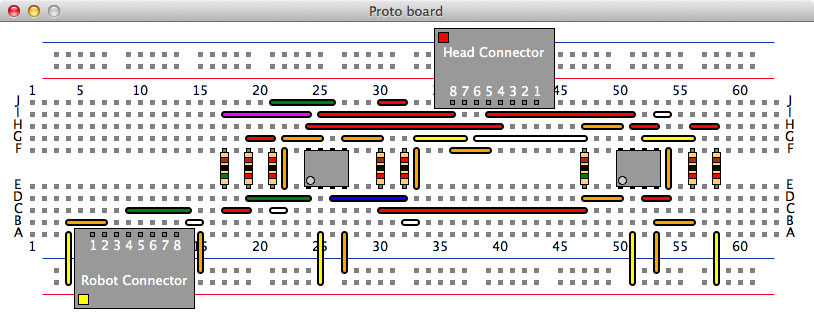
\includegraphics[width=\textwidth]{Images/exemplar_all_pairs.png}
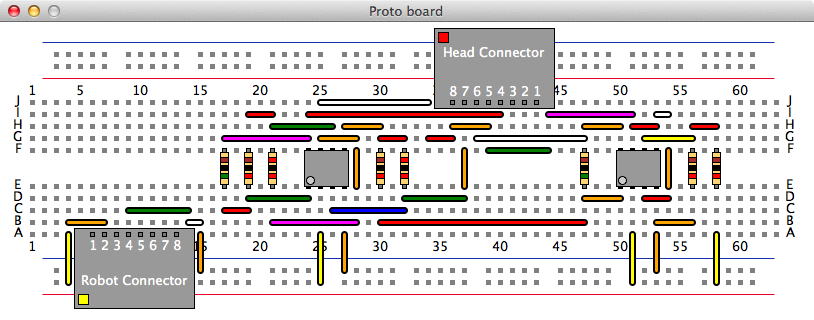
\includegraphics[width=\textwidth]{Images/exemplar_per_node_increasing.png}
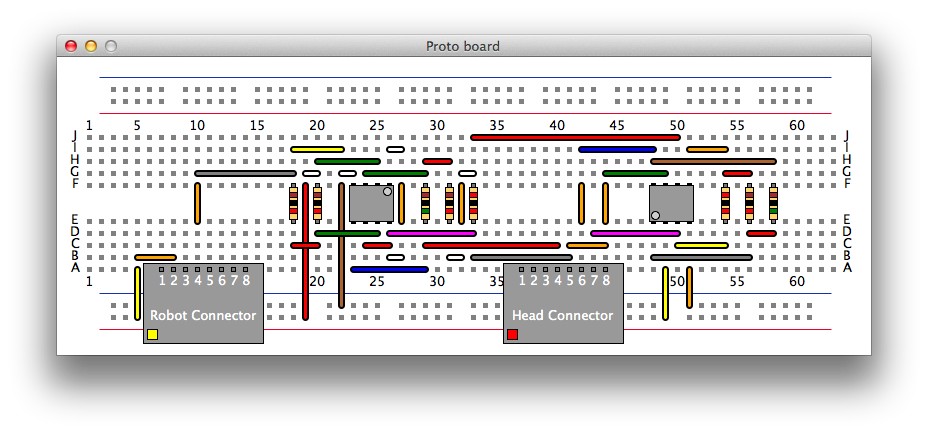
\includegraphics[width=\textwidth]{Images/exemplar_per_node_decreasing.png}
\end{center}
\end{figure}
\begin{figure}
\begin{center}
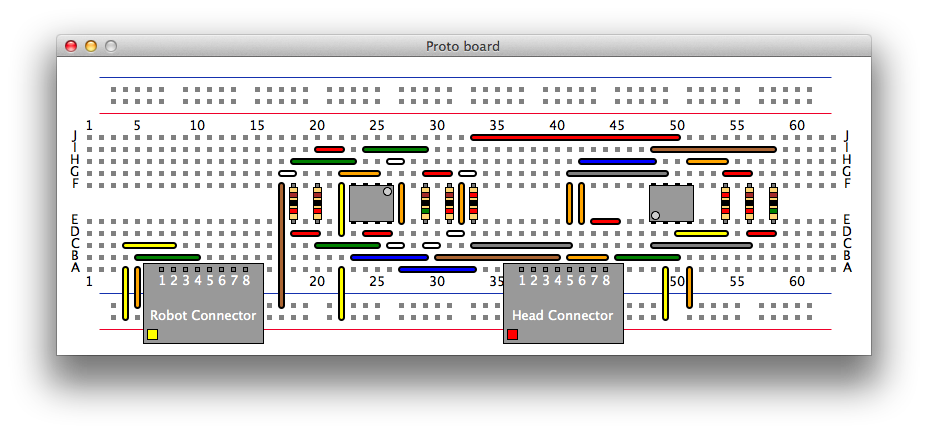
\includegraphics[width=\textwidth]{Images/exemplar_per_pair_increasing.png}
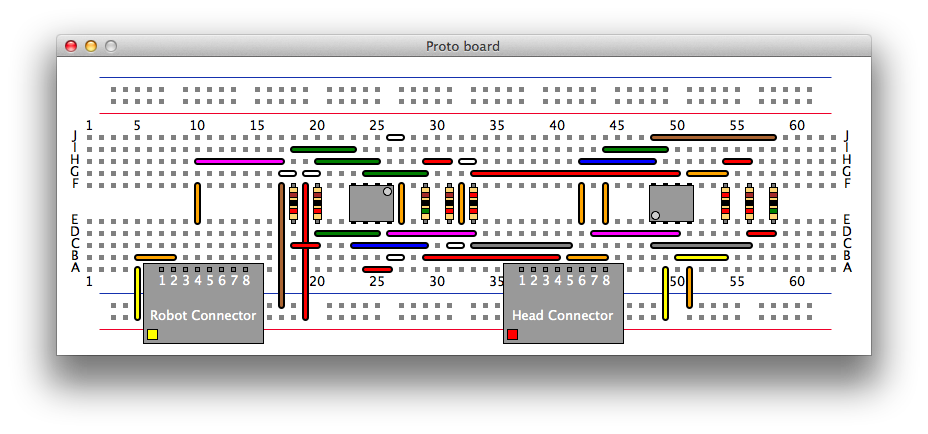
\includegraphics[width=\textwidth]{Images/exemplar_per_pair_decreasing.png}
\caption{All-pairs vs. Per-node, increasing vs. Per-node, decreasing vs.
Per-pair, increasing vs. Per-pair, decreasing.}
\end{center}
\end{figure}

\subsection{Comparing resistor treatments}

We now look at the two alternative treatments for wires: as components vs. as
wires. From Figures \ref{fig:resistor_success} and \ref{fig:resistor_success_trend}
and Table \ref{tb:resistor_success}, we observe that treating resistors as wires
results in a considerably smaller success rate than treating resistors as
components. Recall that the wiring method used here is per-pair, decreasing wiring.
When treating resistors as wires, we get more location pairs to connect.
The key difference for
the location pairs that correspond to resistors is that in connecting the given
pair of locations with wires, one of the wires is required to have length $3$,
the length of a resistor. Intuitively, this restriction should make the search
harder, and the data we have obtained suggests that the search is indeed
significantly more difficult with the restriction than without.

When we treat resistors as wires, and the search does succeed, we observe from
Figure \ref{fig:resistor_time_trend} that it takes more time than treating
resistors as wires, as expected.

Finally we look at the quality of layouts produced by the two methods. First,
we observe from Figure \ref{fig:resistor_quality_trend} that treating resistors
as wires produces layouts with fewer wires and smaller total length of wires
than treating resistors as components. This is certainly expected because each
resistor can be suitably placed to require fewer wires than would be required
if we forced the resistor to reside in the middle strip of the protoboard. We
do note, however, that treating resistors as wires results in more wire crosses
despite requiring fewer wires, especially as circuit complexity increases. This
can be attributed to the fact that treating resistors as wires is likely to
produce more compact layouts in which wire crosses are more likely to happen
than the spreadout settings we force when we treat resistors as components.

In this comparison, we can easily state that, with a limited search (i.e. with
a search in which we have a limited number of states to expand), treating
resistors as components is a better strategy than treating resistors as wires
based on the big difference in success rate.

\begin{figure}
\begin{center}
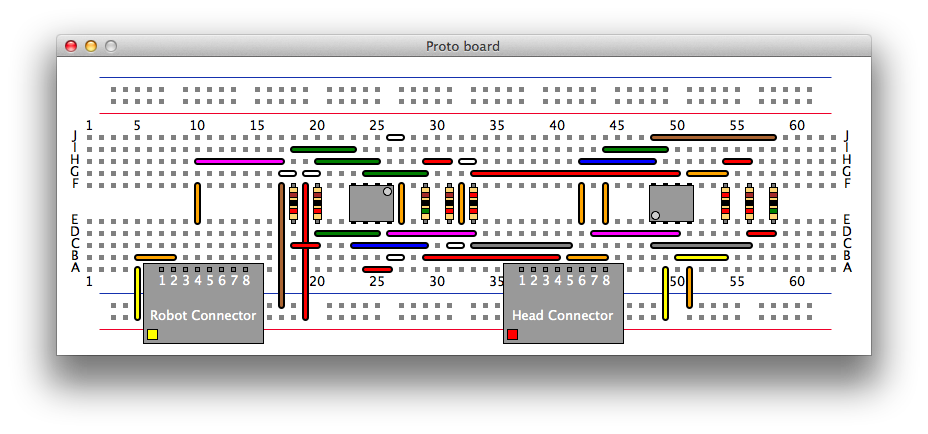
\includegraphics[width=\textwidth]{Images/exemplar_per_pair_decreasing.png}
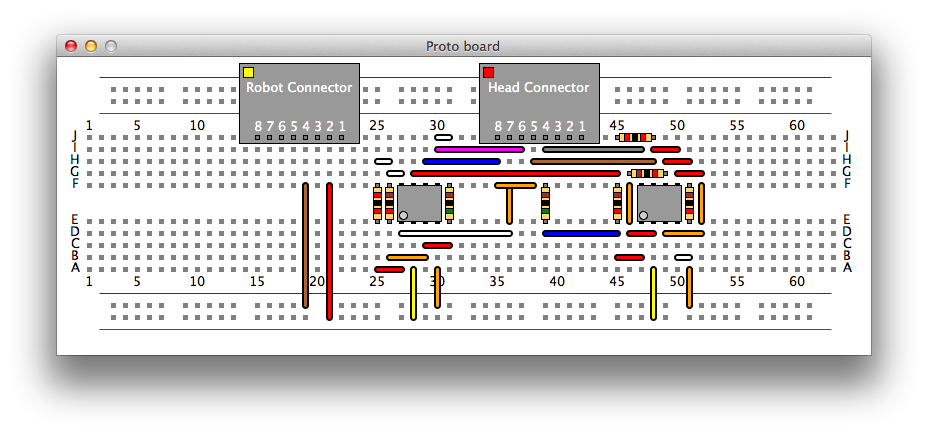
\includegraphics[width=\textwidth]{Images/exemplar_resistors_as_wires.png}
\caption{Resistors as components vs. Resistors as wires.}
\end{center}
\end{figure}

\subsection{Comparing search methods}

We now compare our two alternative search algorithms: $A*$ and Best First Search.
Let us start by comparing success rates. Figures \ref{fig:search_success} and
\ref{fig:search_success_trend} and Table \ref{fig:search_success} present the
appropriate data. We clearly observe that Best First Search is much more
successful than $A*$. $98\%$ of the test circuits were solved at least $8$ times
out of $10$ when we used Best First Search, versues $85\%$ when we used $A*$.
This result is not surprising because Best First Search hungrily hunts for
layouts that satisfy the connection requirements without caring for the
aesthetics of the layouts. Hence, Best First Search is much less succeptible to
the $300$ states to expand restriction than $A*$. The fact that the quality of
the results we get from Best First Search are worse
is clearly evident from Figure \ref{fig:search_quality_trend}. Most importantly, the
number of wire crosses in the layouts produced by Best First Search are markedly
greater than the number of wire crosses in the layouts produced by $A*$. We also
observe that the total wire length is greater when using Best First Search. The
fact that Best First Search settles for any layout that satisfies the connection
requirements suggests that it should finish more quickly in addition to being
more successful. Firgure \ref{fig:search_time_trend} supports exactly this
expectation.

Our choice of a search algorithm forces us to consider a treadoff between quick
success and quality. If we choose Best First Search, most runs will be successful
and terminate quickly, but will produce very poor results. If we choose $A*$,
not as many runs will be successful, and the successful runs will take longer to
terminate, but we will get much better layouts.

\begin{figure}
\begin{center}
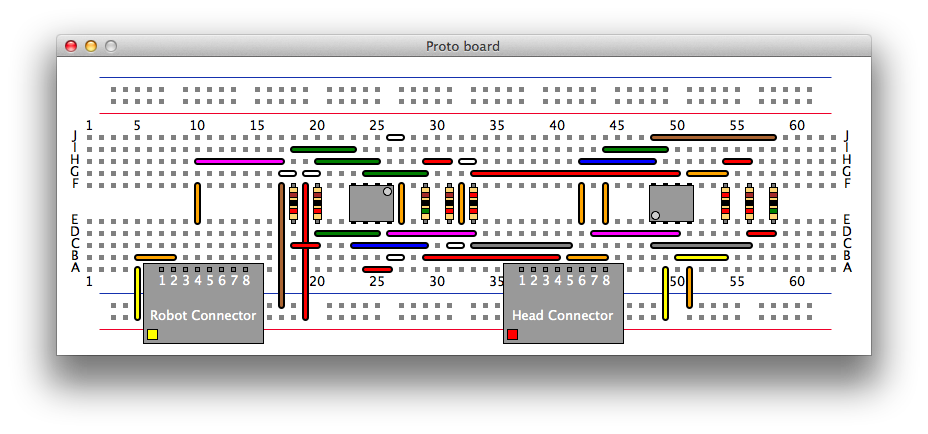
\includegraphics[width=\textwidth]{Images/exemplar_per_pair_decreasing.png}
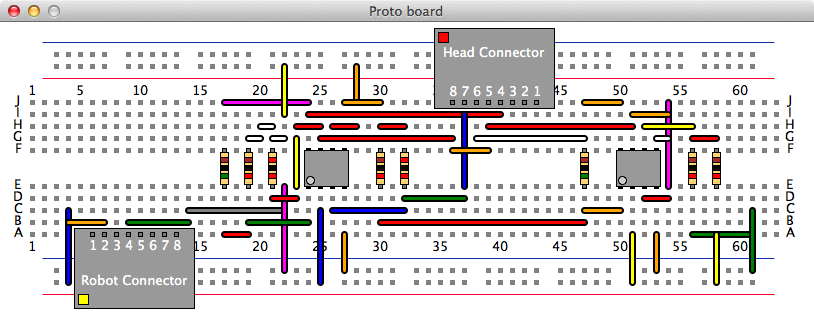
\includegraphics[width=\textwidth]{Images/exemplar_best_first.png}
\caption{$A*$ vs. Best First Search.}
\end{center}
\end{figure}

\subsection{Putting them all together}
\label{sec:method_combination}

\section{Remarks}

\textit{Why are these results encouraging? What are their implications? Relate
back to Introduction to Thesis. What could have been done differently?}

\appendix
\chapter{TODO(mikemeko)}

\clearpage
\newpage

%% This defines the bibliography file (main.bib) and the bibliography style.
%% If you want to create a bibliography file by hand, change the contents of
%% this file to a `thebibliography' environment.  For more information 
%% see section 4.3 of the LaTeX manual.
\begin{singlespace}
\bibliography{main}
\bibliographystyle{plain}
\end{singlespace}

\end{document}

